%!TEX root = ../main.tex

\section{Implementation}
\label{s:implementation}

\begin{figure}
	\plaatje{Pas de kleuren aan, pas het font aan, maak de pipelines verticaal, laat de twee teseelations shaders zien, geef alle blokjes dezelfde stijl, met tikz maken?}
	\centering
	\begin{subfigure}{\columnwidth}
		\centering
		
\includegraphics[width=\columnwidth]{content/img/implementation/pipeLineOld.png}
		\caption{The graphics pipeline of OpenGL version 1.3 (2001).}
		\label{fig:implementation:pipeline:old}
	\end{subfigure}
	\begin{subfigure}{\columnwidth}
		\centering
		
\includegraphics[width=\columnwidth]{content/img/implementation/pipeLineNew.png}
		\caption{The graphics pipeline of OpenGL version 4.1 (2010).}
		\label{fig:implementation:pipeline:new}
	\end{subfigure}	
	\caption{A schematic overview of the programmable parts of the \subref{fig:implementation:pipeline:old} 1.3 and \subref{fig:implementation:pipeline:new} 4.1 OpenGL graphics pipelines. Each rounded rectangle represents one programmable shader.}
	\label{fig:implementation:pipeline}
\end{figure}

A schematic overview of both the OpenGL pipeline at the time of the publication of the paper and the current pipeline are presented in \cref{fig:implementation:pipeline}. These images show that since \citeyear{vlachos2001curved} three new shaders have been introduced into the pipeline, namely the tessellation control, tessellation evaluation and the geometry shader. 

Since only the tessellation shaders are relevant for point-normal triangles we discuss those in more detail in section \ref{ss:implementation:pipeline}. Section \ref{ss:implementation:tcs} through section \ref{ss:implementation:tes} present our implementation of point-normal triangles per discussed tessellation stage. 

\subsection{Tessellation in OpenGL}
\label{ss:implementation:pipeline}

	% Tesselation:
	A schematic overview of tessellation in OpenGL is presented in \Cref{fig:implementation:tessellationPipeline}.
	% Tesselation control
	% Invoked for
	The tessellation control shader (TCS) is invoked once for each vertex in the input patch, which is a triangle in our case. 
	% What does it do
	One of the functions of the tessellation control shader is to set the inner and the outer tessellation levels. Furthermore the TCS can compute additional information about the vertices in the input patch. 
	% Output:
	As can been seen in \cref{fig:implementation:tessellationPipeline} the TCS passes additional information about that patch along to the tessellation evaluation shader (TES) via the output patch. The set inner and outer tessellation levels are sent to the tessellation primitive generator (TPG) \cite{wolff2013opengl}.

	The TPG generates a number of new primitives based on the tessellation levels. How these primitives are generated depends on the selected edge tessellation spacing algorithm. Equal spacing results in evenly divided edges, whereas fractional spacing allows for two shorter edges in the subdivision for more stable interpolation under changing tessellation levels \cite{wolff2013opengl,openGL41Core}. In the case of triangles the barycentric coordinates of the vertices of the newly generated primitives are passed to the TES, as shown in \cref{fig:implementation:tessellationPipeline}.

	% Tesselation evaluation
	% Invoked for
	The tessellation evaluation shader (TES) is executed for each vertex that is generated by the TPG. 
	% Input:
	It receives the coordinates of this vertex in parameter space and the output of the TCS, as is illustrated in \cref{fig:implementation:tessellationPipeline}. 
	% What does it do
	Based on this information it computes the position of the current vertex. 
	% Output:	
	The computed data are passed to the next shader in the pipeline, either the geometry shader or the fragment shader, see \cref{fig:implementation:pipeline:new} \cite{wolff2013opengl}.

	\begin{figure}
		\centering
		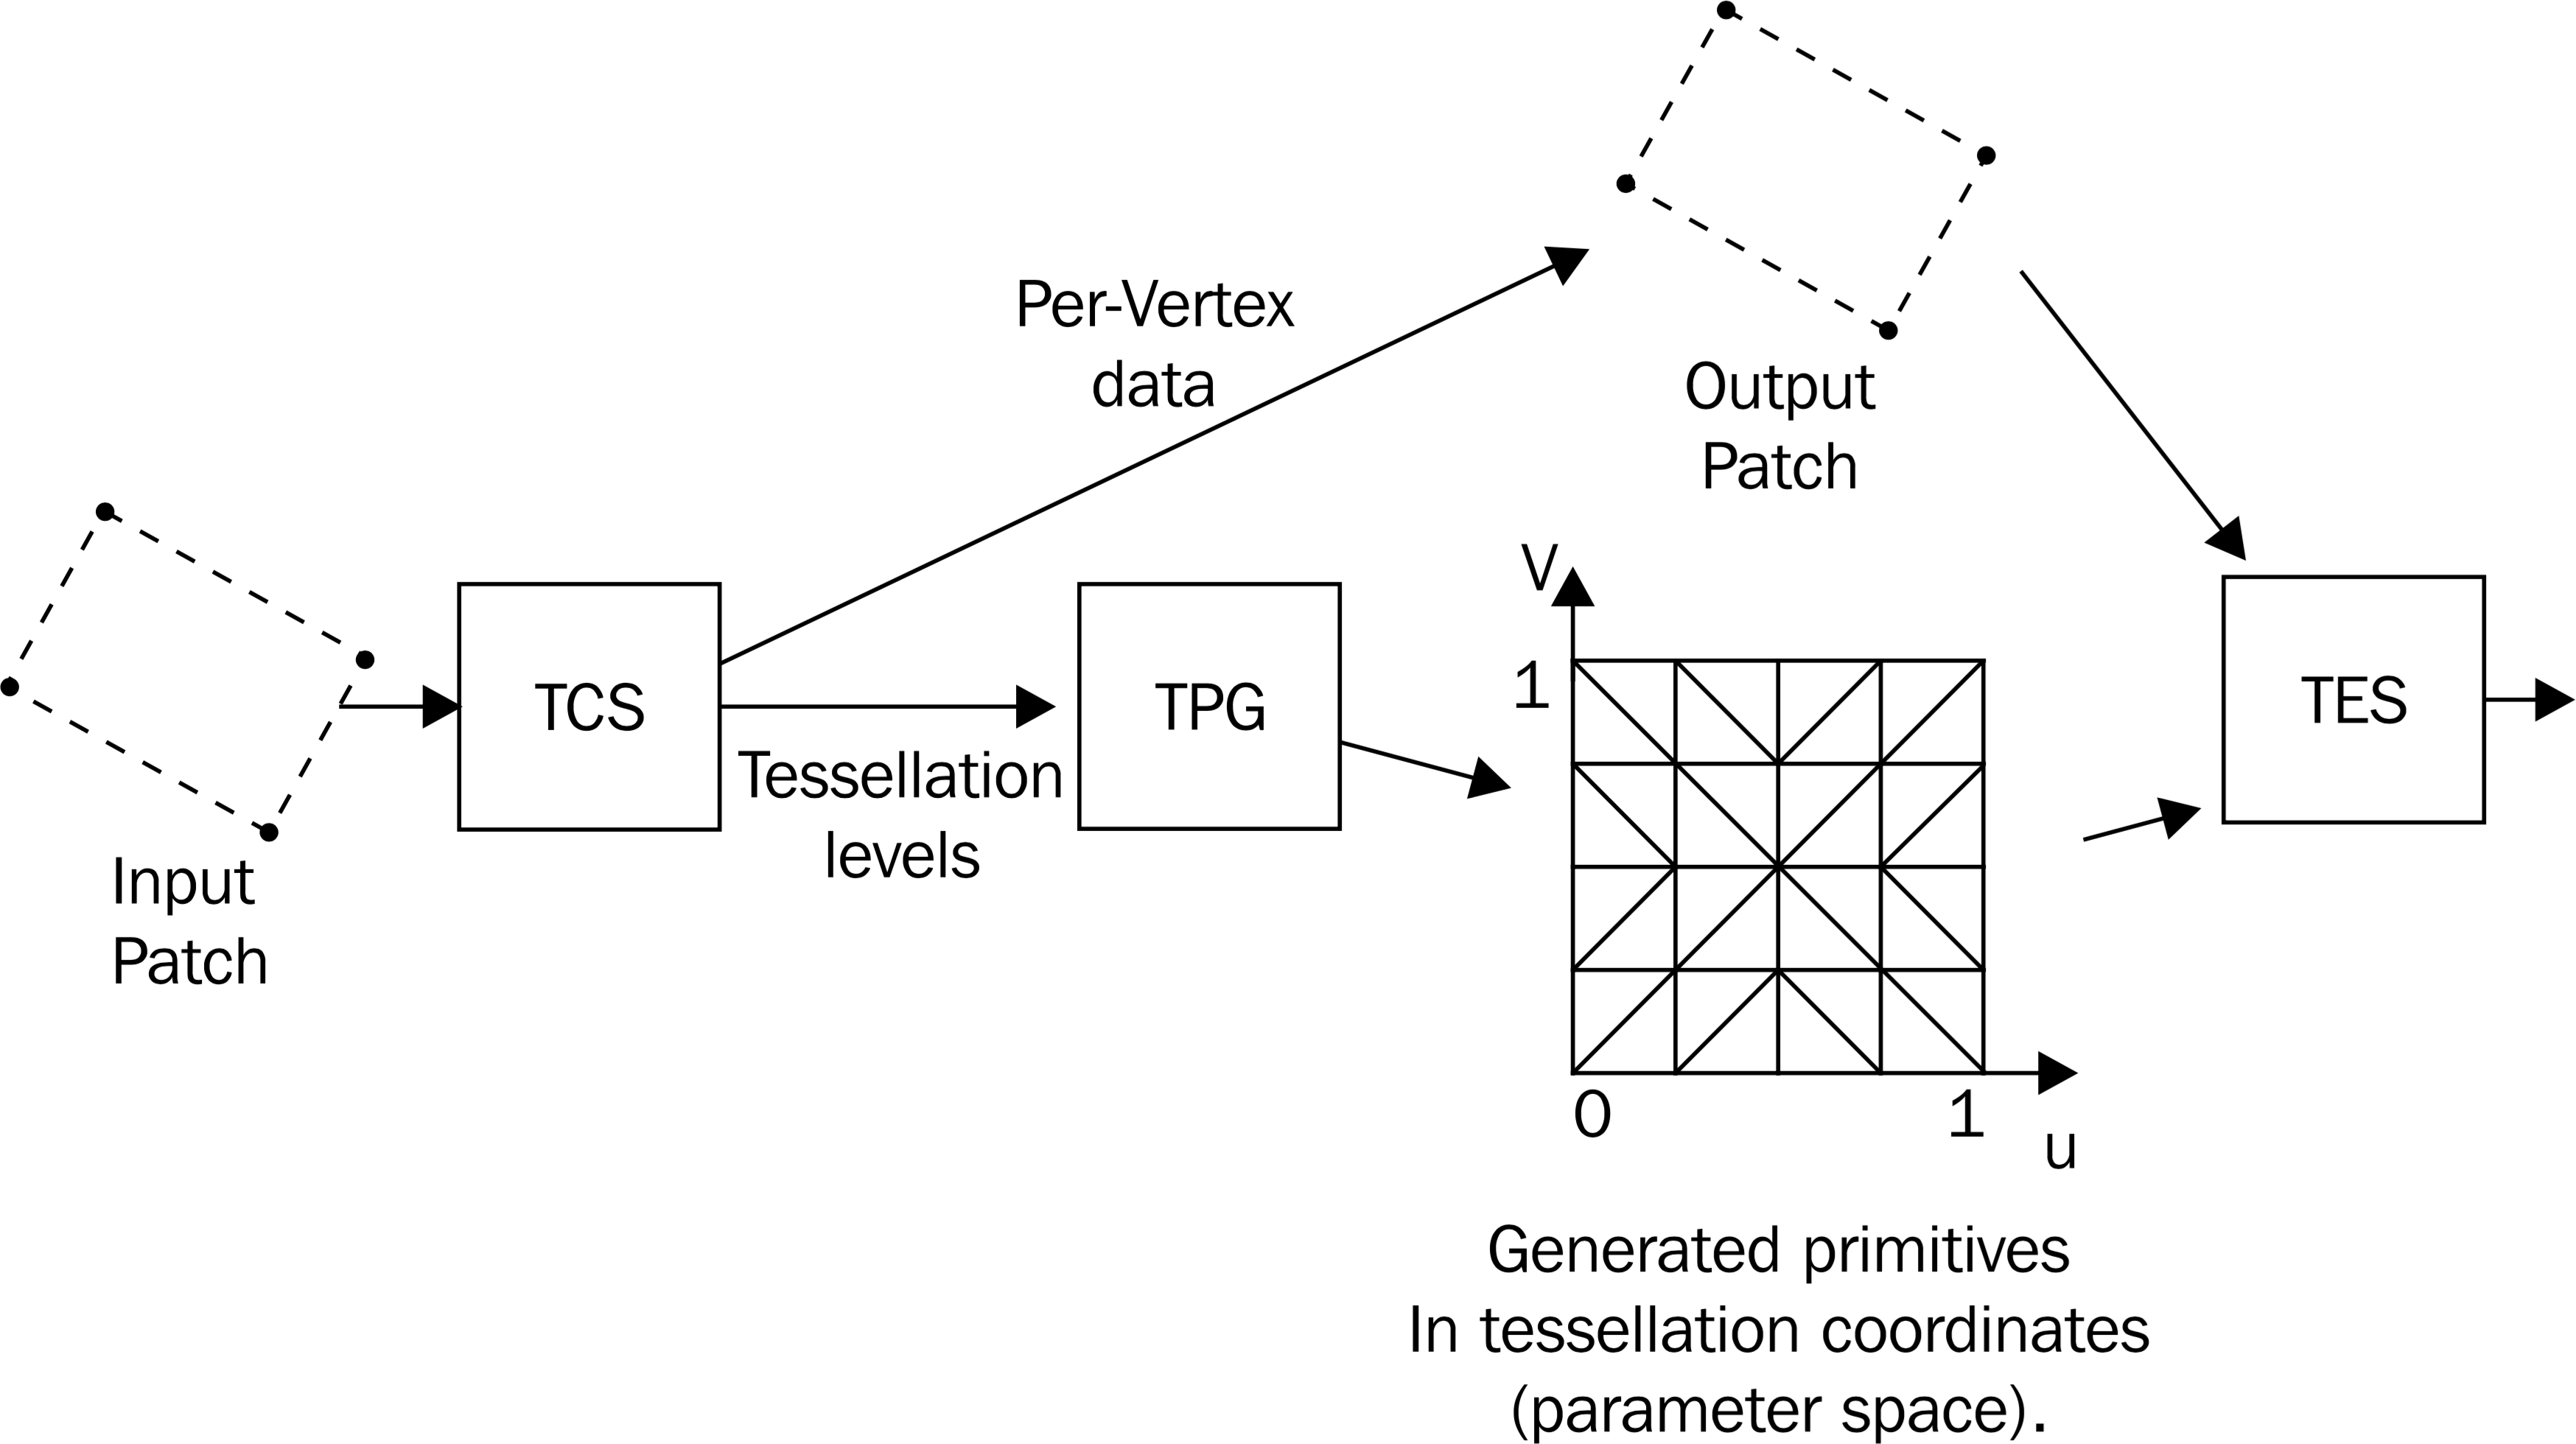
\includegraphics[width=\columnwidth]{content/img/implementation/tesselationPipeline.png}
		\caption{An overview of the tessellation part of the OpenGL render pipeline. Note that in the case of point-normal triangles the input patches, generated primitives and output patches are triangles, not quads. Illustration taken form \textcite{wolff2013opengl}.}
		\label{fig:implementation:tessellationPipeline}
	\end{figure}

\subsection{Tessellation Control Shader}
\label{ss:implementation:tcs}
	% Input
	The TCS receives both the normals and the positions of the vertices of the input patch, in our case, a single triangle. 
	%Computation:
		% Geometry
		Using these it computes the cubic Bézier patch that defines the geometry of the point-normal triangle according to equation \eqref{eq:method:cubic_bezier_patch}.
		% Fake normals
		If `fake' normals are used their control net is computed as well. 
		% Real normals
		The `real' normals need no computations in the tessellation control shader.

		We parallelize the computations of the $x$, $y$ and $z$ component of the vertices of the output patch by using the \texttt{invocation\_ID} to select which component of the output patch to compute. For example if the TCS is invoked for the second vertex of an input patch, i.e. \texttt{invocation\_ID} = 2, we compute the $y$ component of all the vertices of the output patch. This only works since the number of vertices of the input patch is equal to the dimensionality of the positions of the vertices of the output patch.

		There are two alternative ways to compute the output patch. One method is by only computing the output data for e.g. the first vertex. This ensures that no computations are performed twice, however it also means that a lot of threads are waiting for the threads that happened to received the first vertex of a input patch to finish.  
		%
		Alternatively one could always compute all vertices of the output patch, independent of the \texttt{invocation\_ID}. This results in a lot of unnecessary computations, but removes the branching required to only compute the control net if the \texttt{invocation\_ID} has a specific value. Neither of these methods are more efficient than the one we used. A downside of our method is that one has to construct the vectors that represent the vertices of the control net in the tessellation evaluation shader. 

		Other than computing the control nets this shader also sets the inner and outer tessellation levels for the Tessellation Primitive Generator. 
%Output
	The control nets are output to the tessellation evaluation shader whereas the tessellation levels are sent to the tessellation primitive generator. 

\begin{figure}
	\plaatje{Overtrekken in illustrator, 'nough said.}
	\centering
	\begin{subfigure}[b]{0.18\columnwidth}
		\centering
		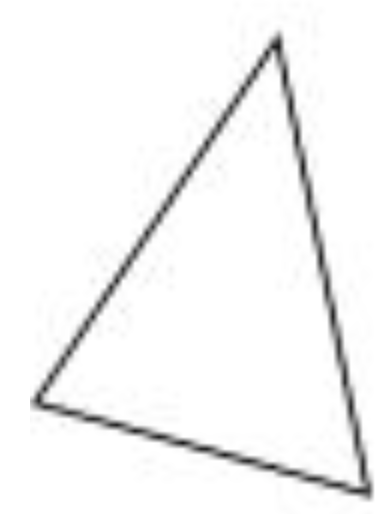
\includegraphics[width=\textwidth]{content/img/implementation/tessellation_input.png}
		\caption{Input}
		\label{fig:implementation:step:input}
	\end{subfigure}
	\begin{subfigure}[b]{0.18\columnwidth}
		\centering
		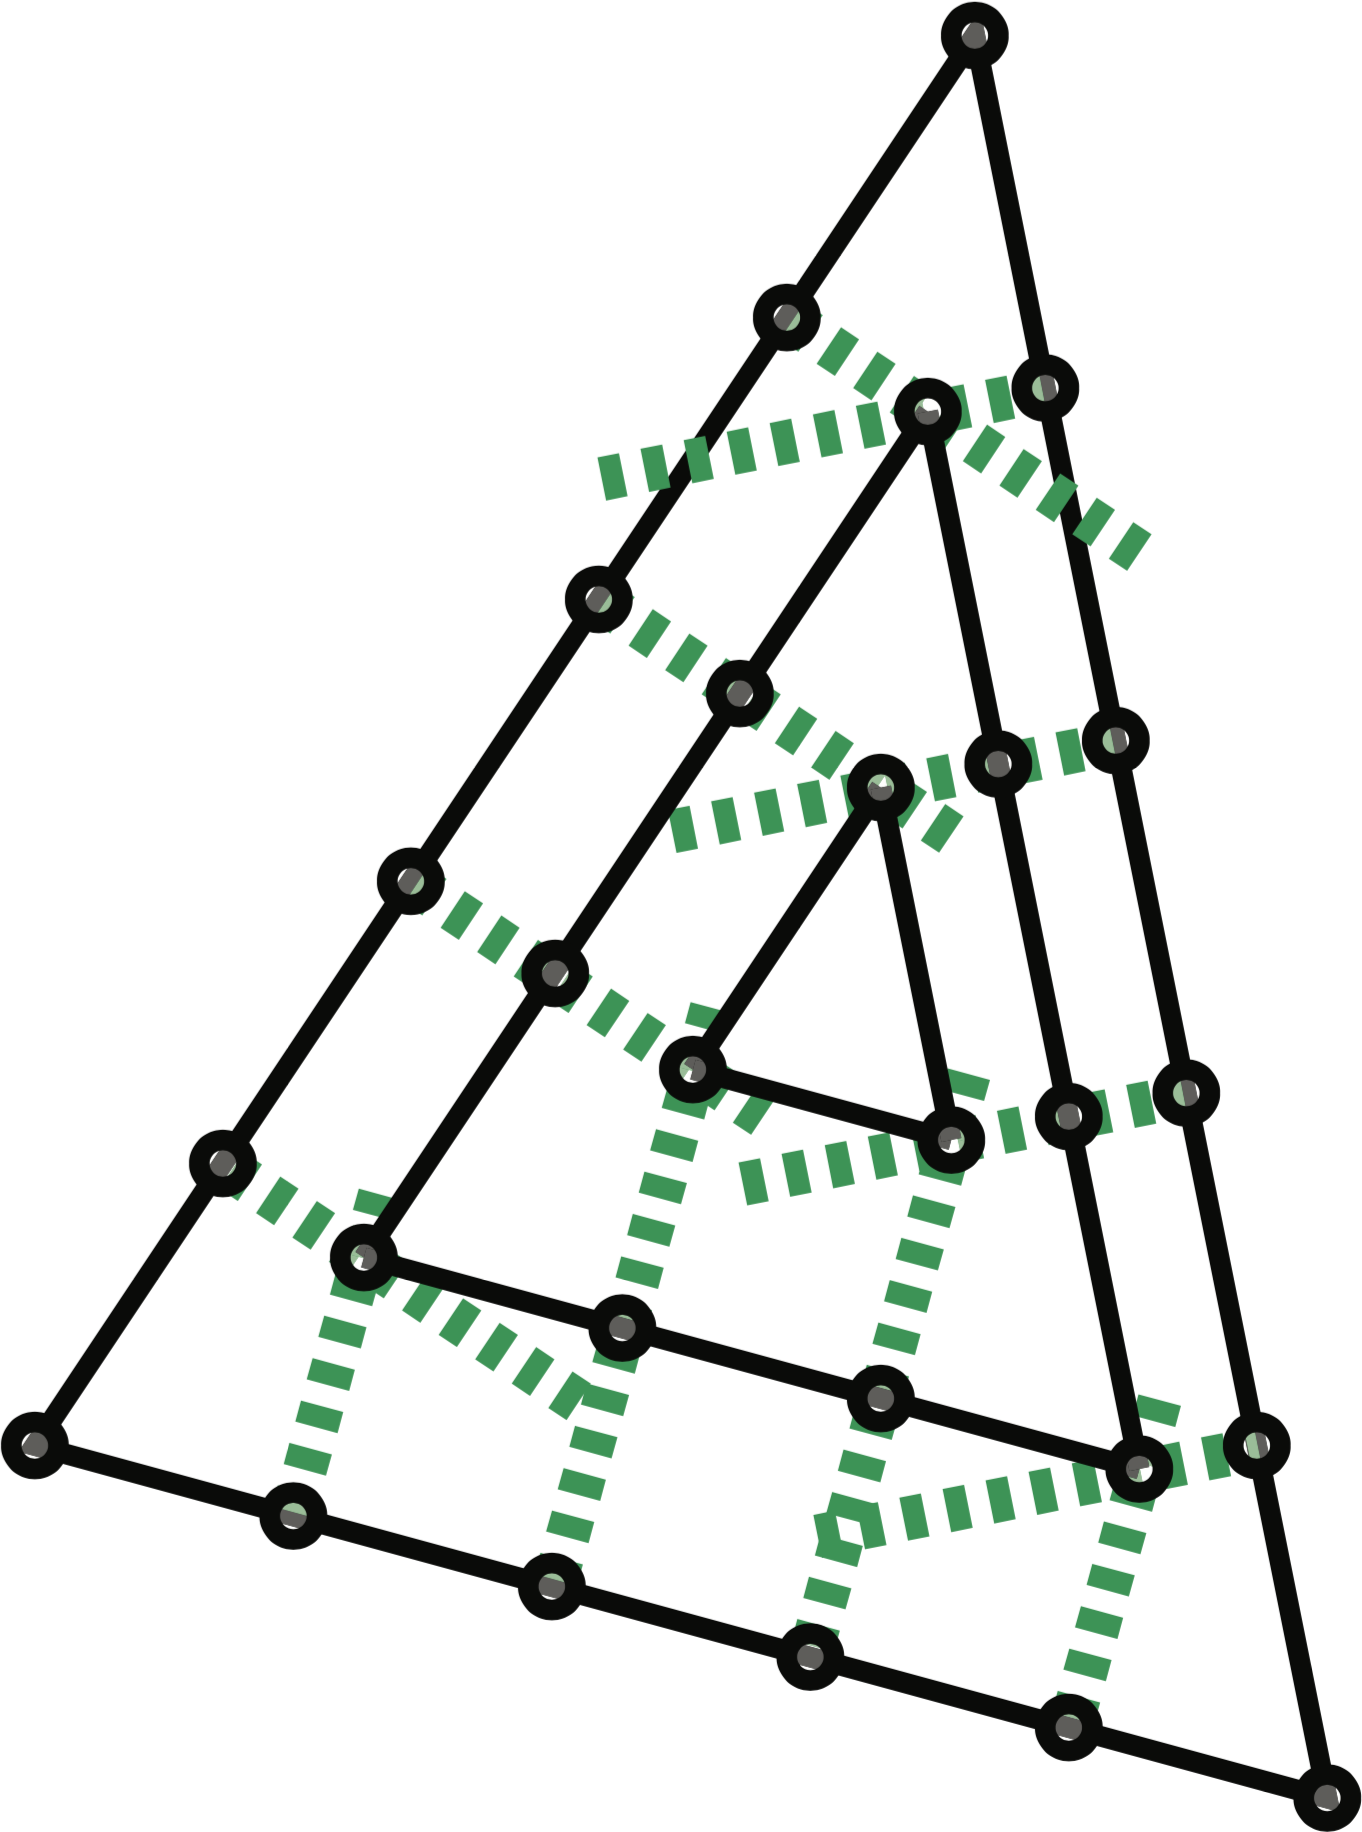
\includegraphics[width=\textwidth]{content/img/implementation/tessellation_1.png}
		\caption{Step \ref{it:implementation:1}}
		\label{fig:implementation:step:1}
	\end{subfigure}	
	\begin{subfigure}[b]{0.18\columnwidth}
		\centering
		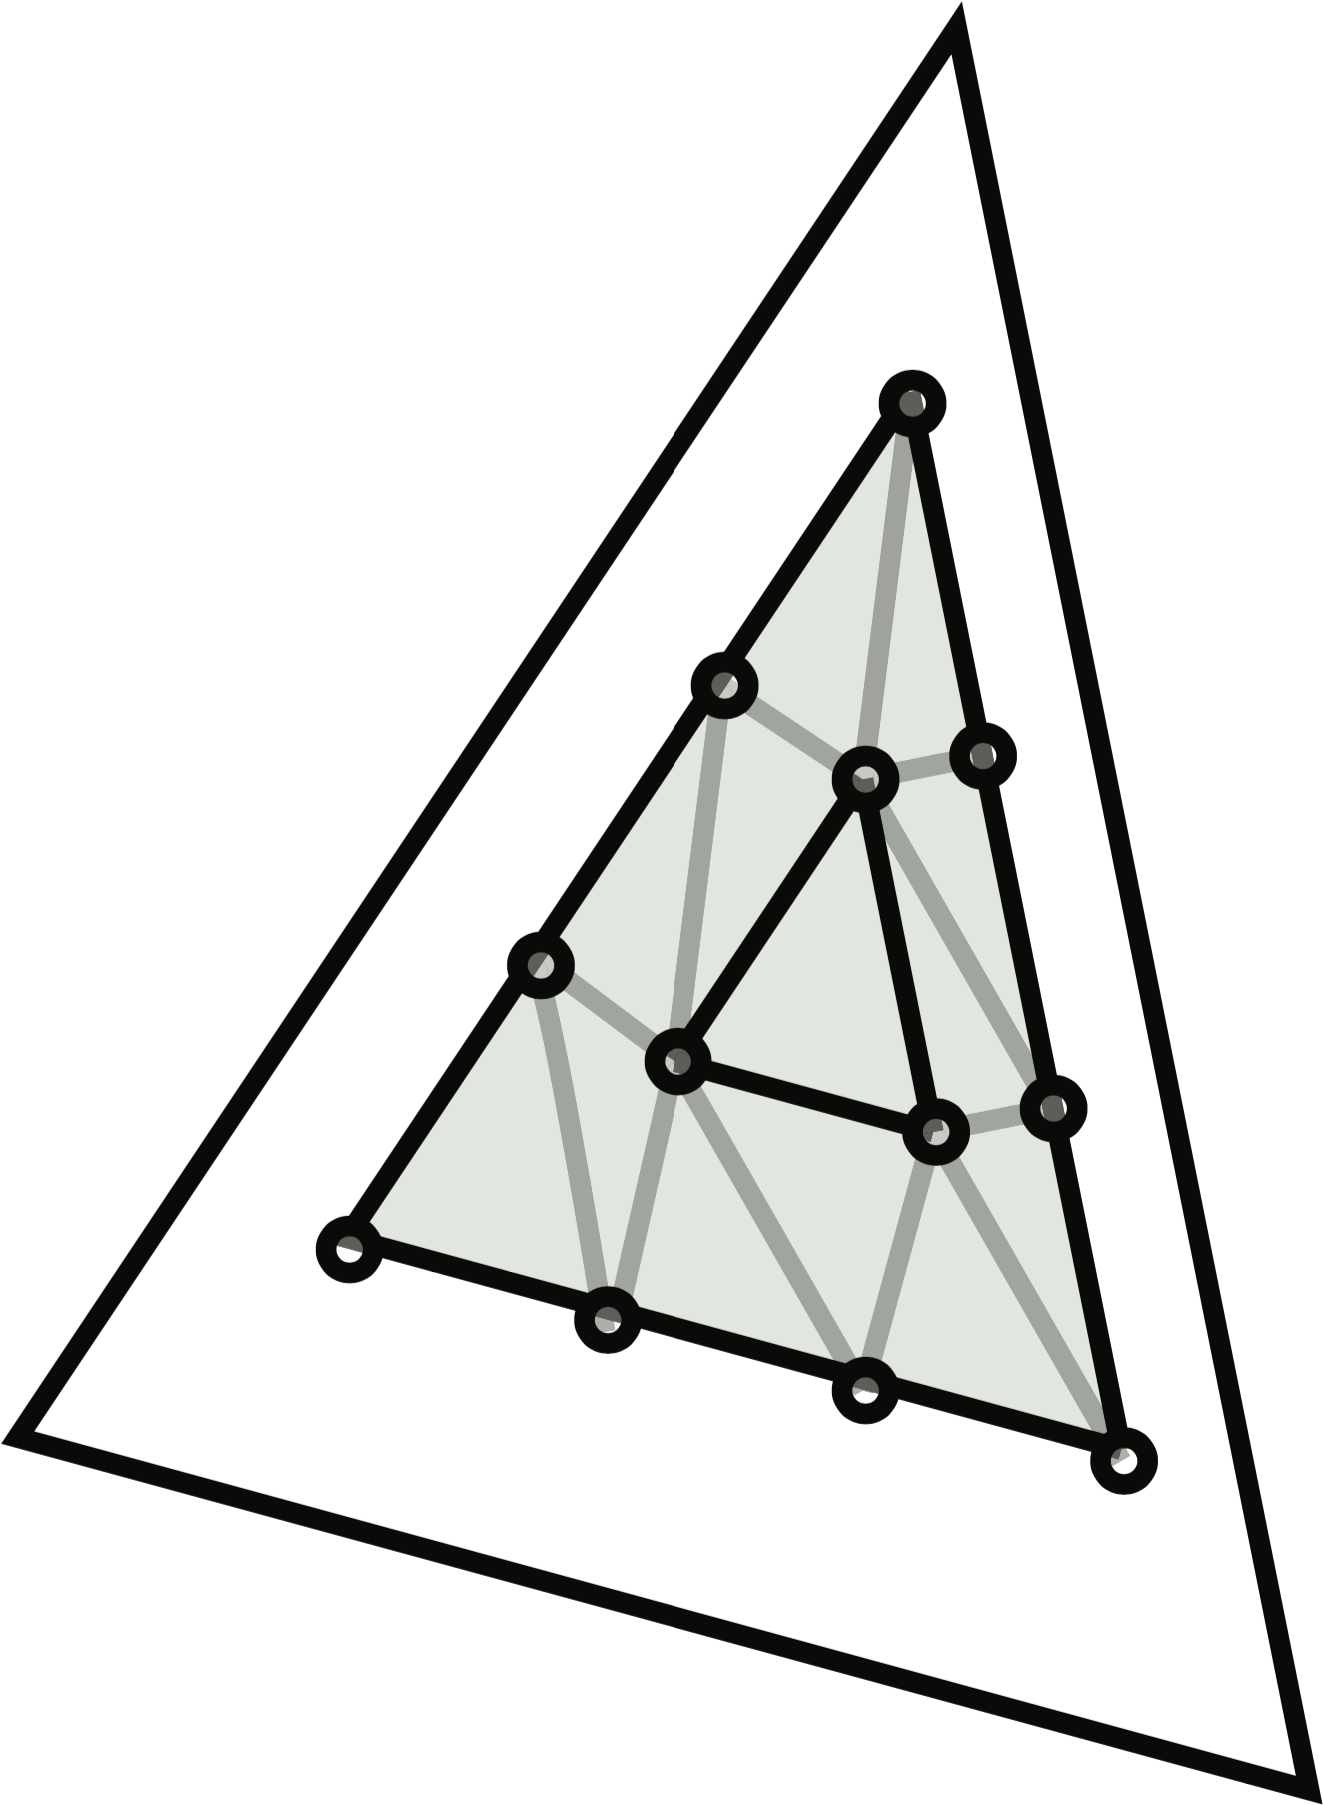
\includegraphics[width=\textwidth]{content/img/implementation/tessellation_2.png}
		\caption{Step \ref{it:implementation:2}}
		\label{fig:implementation:step:2}
	\end{subfigure}		
	\begin{subfigure}[b]{0.18\columnwidth}
		\centering
		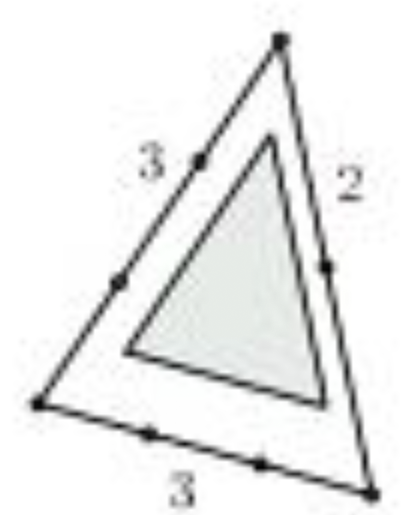
\includegraphics[width=\textwidth]{content/img/implementation/tessellation_3.png}
		\caption{Step \ref{it:implementation:3}}
		\label{fig:implementation:step:3}
	\end{subfigure}		
	\begin{subfigure}[b]{0.18\columnwidth}
		\centering
		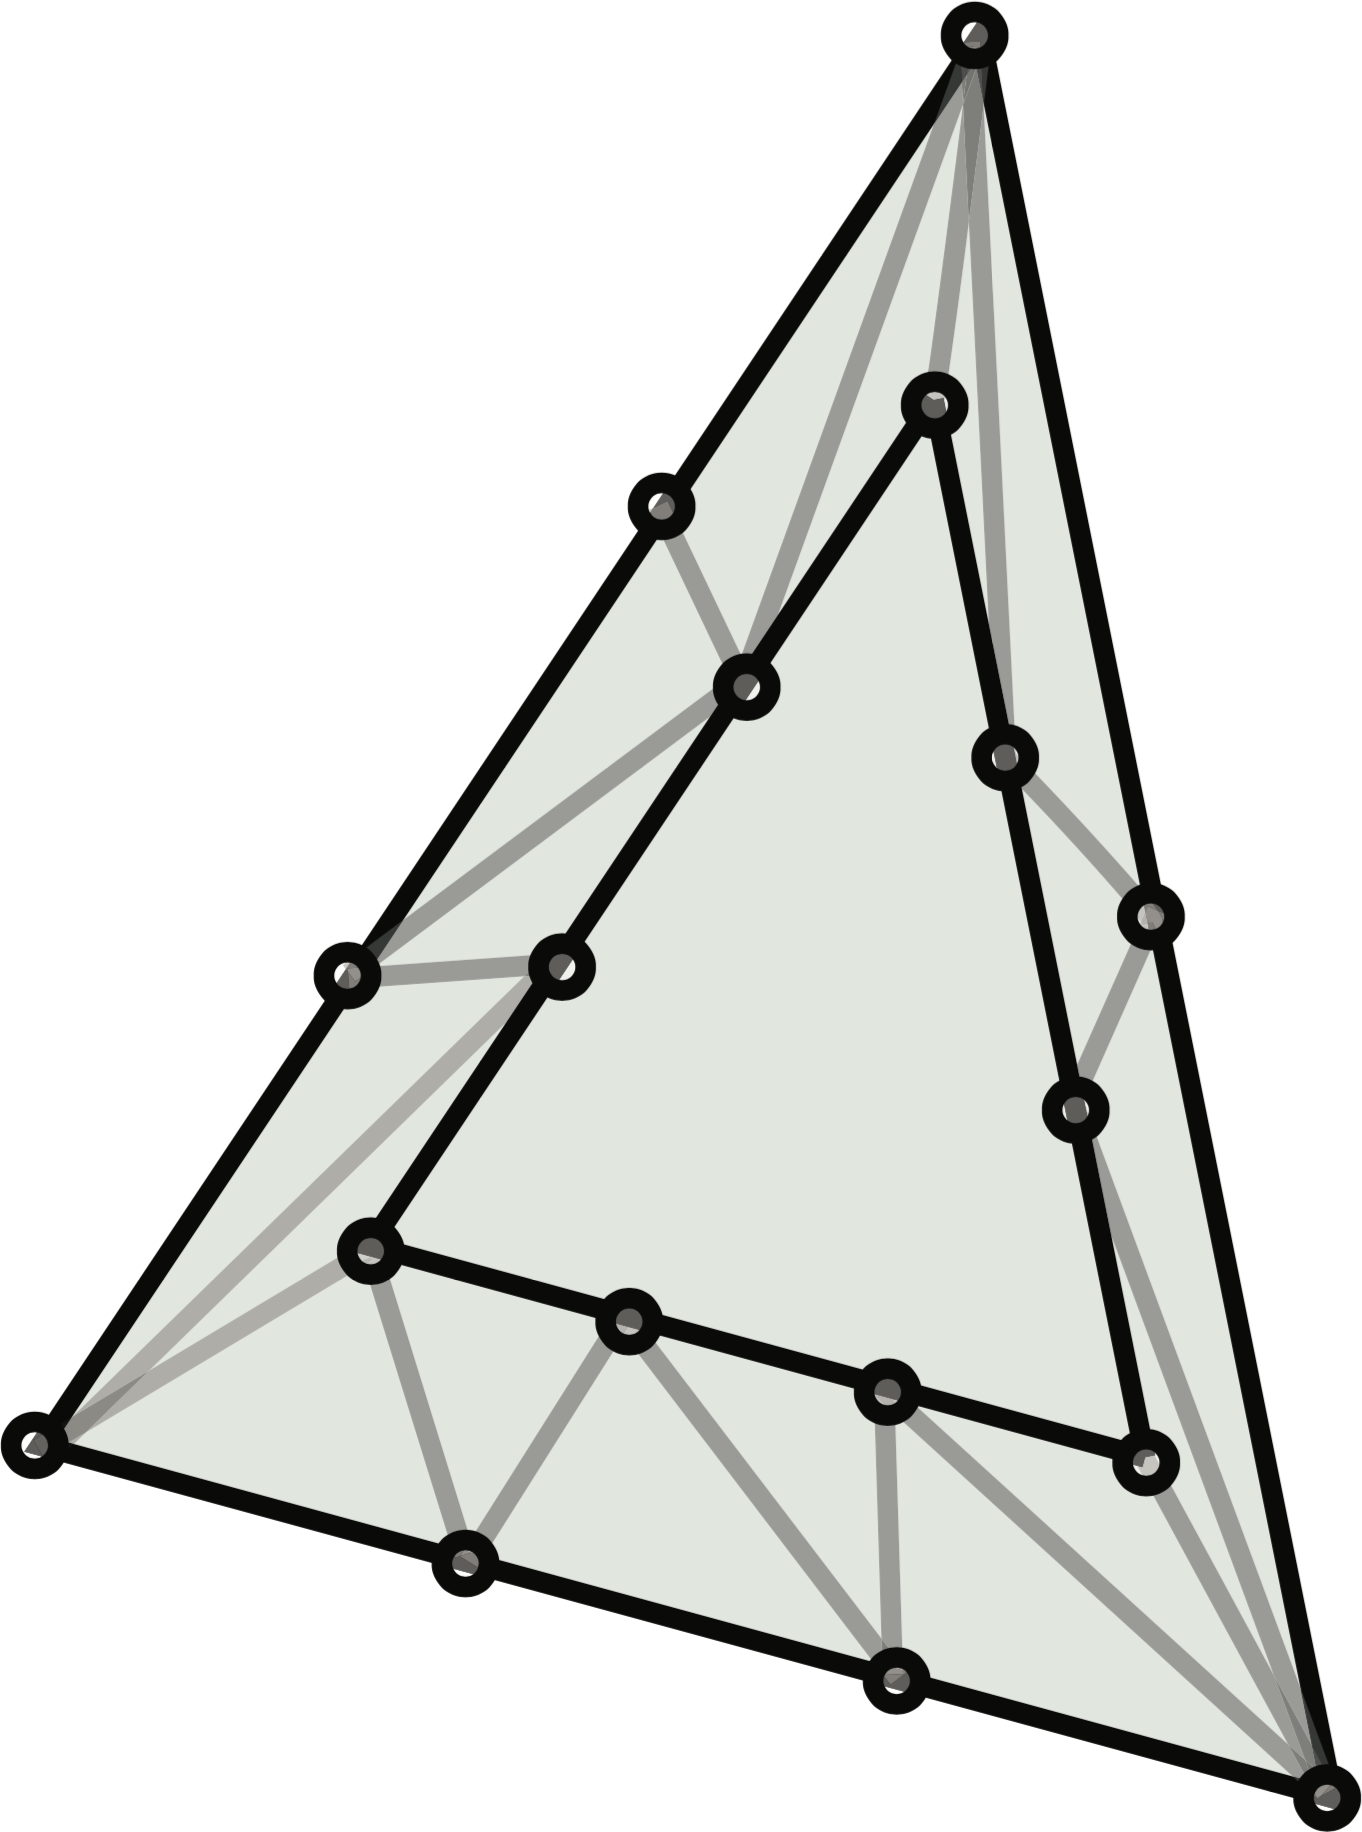
\includegraphics[width=\textwidth]{content/img/implementation/tessellation_4.png}
		\caption{Step \ref{it:implementation:4}}
		\label{fig:implementation:step:4}
	\end{subfigure}		
	\caption{Generation of primitive using the TPG from OpenGL.}
	\label{fig:implementation:step}
\end{figure}

\subsection{Tessellation Primitive Generator}
\label{ss:implementation:tpg}
	The tessellation primitive generator is not programmable, we can however control its output via some parameter, most notably the tessellation levels and the edge tessellation spacing algorithm. The TPG tessellates an input triangle, see \cref{fig:implementation:step:input}, according to these steps \cite{cozzi2012opengl}:
		\begin{enumerate}[label=(\roman*)]
			\item \label{it:implementation:1} The patch is divided into the same number of concentric triangles as the inner tessellation level, see \cref{fig:implementation:step:1}.
			\item \label{it:implementation:2} The spaces between the concentric triangles, except the outer triangle, are subdivided intro triangles, see \cref{fig:implementation:step:2}.
			\item \label{it:implementation:3} The outer edges of the triangles are decomposed in smaller edges according to the outer tessellation level, see \cref{fig:implementation:step:3}.
			\item \label{it:implementation:4} The outer ring of triangles is subdivided into triangles by connecting the vertices from the inner triangles with those of the other triangles, see \cref{fig:implementation:step:4}.
		\end{enumerate}
	A triangle that is tessellated with fractional spacing, and an inner and outer tessellation level of $4.0$ is presented in \cref{fig:implementation:tessellatedTriangle}. It should be noted that the resulting tessellation is different than the subdivision of triangles proposed by \citeauthor{vlachos2001curved}. 

	We opted for fractional odd spacing to make changes between different tessellation levels as smooth as possible. 

	\begin{figure}
		\centering
		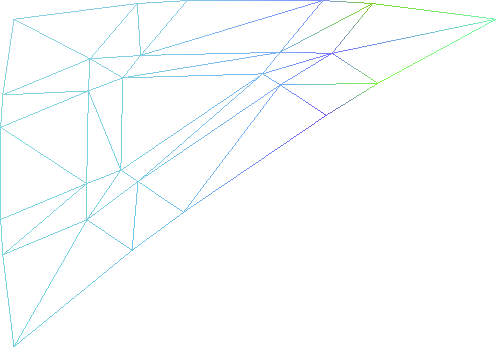
\includegraphics[width=0.5\columnwidth]{content/img/implementation/tesselatedTriangle.png}
		\caption{A single triangle tessellated with both outer and inner tessellation level set to 4.0, and edge tessellation spacing set to \texttt{fractional\_odd\_spacing}.}
		\label{fig:implementation:tessellatedTriangle}
	\end{figure}

\subsection{Tessellation Evaluation Shader}
\label{ss:implementation:tes}
	% Input
	Due to our parallelization the first step in the TES is to extract the control points from the input. 
	% Geometry
	If we have the control nets we determine the positions of the vertices of the flat triangles that will form the final mesh, according to Equation \eqref{eq:method:cubic_bezier_patch}. 
	% Normals
	We compute the normals according to Equation \eqref{eq:method:quadratic_normal_patch} or \todo{reference to the at this point non existing equation.} depending on which normal computation is used. 